\chapter{Logic and quantifiers}
\label{ch:logic}

\section{Predicates and Logical Connectives}
\label{sec:pred}

\noindent{\large \bf Exercises --- \thesection\ }

\begin{enumerate}

\item Design a digital logic circuit (using and, or \& not gates) that 
implements an exclusive or.

\wbvfill

\hint{First, it's essential to know what is meant by the term "exclusive or". This is the interpretation that many people give to the word "or" -- where "X or Y" means either X is true or Y is true, but that it isn't the case that both X and Y are true. This (wrong) understanding of what "or" means is common because it is often the case that X and Y represent complimentary possibilities: old or new, cold or hot, right or wrong... The truth table for exclusive or (often written xor, pronounced "ex-or", symbolically it is usually $\oplus$) is

\begin{tabular}{|c|c|c|} \hline
\rule[-8pt]{0pt}{30pt}$X$ & $Y$ & $X \,\oplus\, Y$ \\ \hline
\rule[-8pt]{0pt}{30pt}$T$ & $T$ & $\phi$ \\ \hline
\rule[-8pt]{0pt}{30pt}$T$ & $\phi$ & $T$ \\ \hline
\rule[-8pt]{0pt}{30pt}$\phi$ & $T$ & $T$ \\ \hline
\rule[-8pt]{0pt}{30pt}$\phi$ & $\phi$ & $\phi$  \\ \hline
\end{tabular}

\noindent So it's true when one, or the other, but not both of its inputs are true.  The upshot of the last sentence is that we can write $X \oplus Y \; \equiv \; (X \lor Y) \land {\lnot}(X \land Y)$.

The above reformulation should help\ldots 

\vfill

}

\workbookpagebreak

\item Consider the sentence 
``This is a sentence which does not refer to itself.''
which was given in the beginning of this chapter as an example.
Is this sentence a statement?  If so, what is its truth value?

\hint{The only question in your mind, when deciding whether a sentence is a statement, should be "Does this thing have a definite truth value?"
Well?

Isn't it just plainly false?}

%\vspace{.5in}
\vfill

\item Consider the sentence ``This sentence is false.''  Is this 
sentence a statement?

\hint{Try to justify why this sentence can't be either true or false.}

\hintspagebreak

%\vspace{.5in}
\vfill

\workbookpagebreak

\item Complete truth tables for each of the sentences 
$(A \land B) \lor C$ and
$A \land (B \lor C)$.  Does it seem that these sentences have
the same logical content?

\hint{

\vfill

A tiny hint here: since the sentences involve 3 variables you'll need truth tables with 8 rows. Here's a template.

\vfill

\begin{tabular}{|c|c|c|c|c|} \hline
\rule[-8pt]{0pt}{30pt}$A$ & $B$ & $C$ & $(A \land B) \lor C$ & $A \land (B \lor C)$ \\ \hline
\rule[-8pt]{0pt}{30pt}$T$ & $T$ & $T$ & \rule{100pt}{0pt} & \rule{100pt}{0pt} \\ \hline
\rule[-8pt]{0pt}{30pt}$T$ & $T$ & $\phi$  & & \\ \hline
\rule[-8pt]{0pt}{30pt}$T$ & $\phi$  & $T$ & & \\ \hline
\rule[-8pt]{0pt}{30pt}$T$ & $\phi$  & $\phi$  & & \\  \hline
\rule[-8pt]{0pt}{30pt}$\phi$  & $T$ & $T$ & & \\ \hline
\rule[-8pt]{0pt}{30pt}$\phi$  & $T$ & $\phi$  & & \\ \hline
\rule[-8pt]{0pt}{30pt}$\phi$  & $\phi$  & $T$ & & \\ \hline
\rule[-8pt]{0pt}{30pt}$\phi$  & $\phi$  & $\phi$  & & \\  \hline
\end{tabular}
}
\vfill

\hintspagebreak
\workbookpagebreak

\item \label{ex:nand_nor} There are two other logical connectives that are
used somewhat less commonly than $\lor$ and $\land$.
These are the \index{Scheffer stroke} Scheffer stroke and the 
\index{Peirce arrow}Peirce arrow
-- written $\vert$ and $\downarrow$, respectively ---  they are 
also known as \index{NAND} NAND and \index{NOR} NOR.

\noindent The truth tables for these connectives are:
\medskip

\begin{tabular}{c|c|c}
$A$ & $B$ & $A \,\vert\, B$ \\ \hline
$T$ & $T$ & $\phi$ \\
$T$ & $\phi$ & $T$ \\
$\phi$ & $T$ & $T$ \\
$\phi$ & $\phi$ & $T$ 
\end{tabular}
\hspace{.25 in} and \hspace{.25 in}
\begin{tabular}{c|c|c}
$A$ & $B$ & $A \downarrow B$ \\ \hline
$T$ & $T$ & $\phi$ \\
$T$ & $\phi$ & $\phi$ \\
$\phi$ & $T$ & $\phi$ \\
$\phi$ & $\phi$ & $T$ 
\end{tabular}
\medskip

Find an expression for $(A\, \land {\lnot}B) \lor C$
using only these new connectives (as well as negation and the
variable symbols themselves).


\hint{Sorry, I know this is probably the hardest problem in the chapter, but I'm (mostly) not going to help...
Just one hint to help you get started: NAND and NOR are the negations of AND and OR (respectively) so, for example, $(X \land Y) \; \equiv \; {\lnot}(A \,\vert\, B)$.}

\textbookpagebreak
\workbookpagebreak


\item \label{IKK} The famous logician \index{Smullyan, Raymond} Raymond Smullyan devised 
a family of logical puzzles around a fictitious place he called 
\index{Knights and Knaves} ``the Island of Knights and Knaves.''  The inhabitants of the island are either knaves, who always make false statements, or knights, who always make truthful statements.  

In the most famous knight/knave puzzle, you are in a room which has only two exits.  One leads to certain death and the other to freedom.  There are two 
individuals in the room, and you know that one of them is a knight and the other is a knave, but you don't know which.   Your challenge is to determine the door which leads to freedom by asking a single question.

\hint{Ask one of them what the other one would say to do.}

\end{enumerate}


\newpage

\section{Implication}
\label{sec:impl}

\noindent{\large \bf Exercises --- \thesection\ }

\begin{enumerate}

\item The transitive property of equality says that if $a=b$ and $b=c$
then $a=c$.  Does the implication arrow satisfy a transitive property?
If so, state it.

\wbvfill

\hint{
I sometimes like to rephrase the implication $X \implies Y$ as ``X's truth forces Y to be true.''  Does that help?
If we know that X being true forces Y to be true, and we also know that Y being true will force Z to be true, what can we conclude?

\vfill

}

\item Complete truth tables for the compound sentences $A \implies B$ and
  ${\lnot}A \lor B$.
  
  \wbvfill
  
\hint{
You should definitely be able to do this one on your own, but anyway, here's an outline of the table:

\begin{tabular}{|c|c|c|c|} \hline
\rule[-6pt]{0pt}{24pt}  $A$ & $B$ & $A \implies B$ & ${\lnot}A \lor B$ \\ \hline
\rule[-6pt]{0pt}{24pt}  $T$ &  $T$ & & \\ \hline
\rule[-6pt]{0pt}{24pt}  $T$ & $\phi$ & & \\ \hline	 	 
\rule[-6pt]{0pt}{24pt}  $\phi$ & $T$ & & \\ \hline
\rule[-6pt]{0pt}{24pt}  $\phi$ & $\phi$ & & \\ \hline
\end{tabular}

\vfill

}

\item Complete a truth table for the compound sentence $A \implies (B \implies C)$ and for the sentence $(A \implies B) \implies C$.  What can you conclude
about conditionals and the associative property?

\wbvfill

\hint{
No help on this one other than to say that the associative property {\bf does not} hold for implications.

\vfill

}

\workbookpagebreak
\hintspagebreak

\item Determine a sentence using the {\em and} connector ($\land$) that
gives the negation of $A \implies B$.

\wbvfill

\hint{Hmmm\ldots This will seem like a strange hint, but if you were to hear a kid at the playground say ``Oh yeah? Well, I did call your mom a fatty and you still haven't clobbered me! Owww! OWWW!!! Stop hitting me!!''

What conditional sentence was he attempting to negate?
}

\item Rewrite the sentence ``Fix the toilet or I won't pay the rent!'' as
a conditional.

\wbvfill

\hint{The way I see it there are eight possible ways to arrange "You fix the toilet" and "I'll pay the rent" (or their respective negations) around an implication arrow.
Here they all are. You decide which one sounds best.

If you fix the toilet, then I'll pay the rent.\newline
If you fix the toilet, then I won't pay the rent.\newline
If you don't fix the toilet, I'll pay the rent.\newline
If you don't fix the toilet, then I won't pay the rent.\newline
If I payed the rent, then you must have fixed the toilet.\newline
If I payed the rent, then you must not have fixed the toilet.\newline
If I didn't pay the rent, then you must have fixed the toilet.\newline
If I didn't pay the rent, then you must not have fixed the toilet.\newline

Some of those are truly strange\ldots
}
\item Why is it that the sentence ``If pigs can fly, I am the king
of Mesopotamia.'' true?

\wbvfill

\hint{Unless we're talking about some celebrity bringing their pet Vietnamese pot-bellied pig into first class with them, or possibly a catapult of some type... The antecedent (the if part) is false, so Yay! I AM the king of Mesopotamia!! Whoo-hooh! What? I'm not? Oh. But the if-then sentence is true. Bummer.}

\item Express the statement $A \implies B$ using the Peirce arrow and/or the
Scheffer stroke. (See Exercise~\ref{ex:nand_nor} in the previous section.)

\wbvfill

\hint{You'll want to use $\vert$, the Scheffer stroke, aka NAND, because it's truth table contains three $T$'s and one $\phi$ -- you'll just need to figure out which of its inputs to negate so as to make that one $\phi$ occur in the second row of the table instead of the first.}

\workbookpagebreak

\item Find the contrapositives of the following sentences.
  \begin{enumerate}
  \item If you can't do the time, don't do the crime.
  \item If you do well in school, you'll get a good job.
  \item If you wish others to treat you in a certain way, you must 
    treat others in that fashion.
  \item If it's raining, there must be clouds.
  \item If $a_n \leq b_n$, for all $n$ and $\sum_{n=0}^\infty b_n$ is a 
convergent series, then $\sum_{n=0}^\infty a_n$ is a convergent series.
  \end{enumerate}

\wbvfill

\hint{
\begin{enumerate}
\item If you do the crime, you must do the time.
\item If you don't have a good job, you must've done poorly in school.
\item If you don't treat others in a certain way, you can't hope for others to treat you in that fashion,
\item If there are no clouds, it can't be raining.
\item If  $\sum_{n=0}^\infty a_n$ is not a convergent series, then either $a_n \leq b_n$, for some $n$ or 
$\sum_{n=0}^\infty b_n$ is not a convergent series.
\end{enumerate}
}
\rule{0pt}{0pt}

\wbvfill

\item What are the converse and inverse of ``If you watch my back, I'll 
watch your back.''?

\wbvfill

\hint{
The converse is ``If I watch your back, then you'll watch my back.''  (Sounds a little dopey doesn't it -- likes its sort of a wishful thinking\ldots)
The inverse is ``If you don't watch my back, then I won't watch your back.''  (Sounds less vapid, but it means the same thing\ldots)
}

\workbookpagebreak

\item The integral test in Calculus is used to determine whether an
infinite series converges or diverges:   Suppose that $f(x)$ is a positive,
decreasing, 
real-valued function with $\lim_{x \longrightarrow \infty} f(x) = 0$, if
the improper integral
$\int_0^\infty f(x)$ has a finite value, then the infinite series 
$\sum_{n=1}^\infty f(n)$ converges.

The integral test should be envisioned by letting the series correspond
to a right-hand Riemann sum for the integral, since the function is decreasing,
a right-hand Riemann sum is an underestimate for the value of the integral,
thus

\[ \sum_{n=1}^\infty f(n) < \int_0^\infty f(x). \]

Discuss the meanings of and (where possible) provide justifications for
the inverse, converse and contrapositive of the conditional statement 
in the integral test.

\wbvfill

\hint{
The inverse says -- if the integral isn't finite, then the series doesn't converge. You can cook-up a function that shows this to be false by (for example) creating one with vertical asymptotes that occur in between the integer $x$-values. Even one such pole can be enough to make the integral go infinite.
The converse says that if the series converges, the integral must be finite. The counter-example we just discussed would work here too.

The contrapositive says that if the series doesn't converge, then the integral must not be finite. If we were allowed to use discontinuous functions, it isn't too hard to come up with an $f$ that actually has zero area under it -- just make f be identically zero except at the integer x-values where it will take the same values as the terms of the series. But wait, the function we just described isn't ``decreasing'' -- which is probably why that hypothesis was put in there!
}

\workbookpagebreak

\item On the Island of Knights and Knaves (see page~\pageref{IKK}) you encounter two individuals named Locke and Demosthenes.  

Locke says, ``Demosthenes is a knave.'' \newline
Demosthenes says ``Locke and I are knights.''

Who is a knight and who a knave?

\wbvfill

\hint{Could Demosthenes be telling the truth?}

\end{enumerate}


\newpage

\section{Logical equivalences}
\label{sec:le}

\noindent{\large \bf Exercises --- \thesection\ }

\begin{enumerate}

\item There are 3 operations used in basic algebra (addition, 
multiplication and exponentiation) and thus
there are potentially 6 different distributive laws.  State
all 6 ``laws'' and determine which 2 are actually valid.
(As an example, the distributive law of addition over multiplication
would look like $x + (y \cdot z) = (x + y) \cdot (x + z)$, this isn't 
one of the true ones.) 

\wbvfill

\hint{
\vfill

These ``laws'' should probably be layed-out in a big 3 by 3 table. Such a table would of course have 9 cells, but we won't be using the cells on the diagonal because they would involve an operation distributing over itself. (That can't happen, can it?)
I'm going to put a few of the entries in, and you do the rest.

\vfill

\begin{tabular}{c|c|c|c|} 
  & \rule{36pt}{0pt} $+$ \rule{36pt}{0pt} & \rule{36pt}{0pt} $\ast$ \rule{36pt}{0pt} & \rule{36pt}{0pt} $\caret$ \rule{36pt}{0pt} \\ \hline
 \rule[-36pt]{0pt}{72pt} $+$ & $\emptyset$ & \parbox{1.4in}{\begin{gather*}x+(y\ast z) \\= (x+y) \ast (x+z)\end{gather*}} & \parbox{1.4in}{\begin{gather*}x+(y^z) \\ = (x+y)^{(x+z)} \end{gather*} } \\ \hline
 \rule[-36pt]{0pt}{72pt} $\ast$ & \parbox{1.4in}{\begin{gather*} x \ast (y+z) \\ = (x \ast y) + (x \ast z)\end{gather*} } & $\emptyset$ &  \\ \hline
 \rule[-36pt]{0pt}{72pt} $\caret$ & & & $\emptyset$ \\ \hline
\end{tabular}

\vfill

\rule{0pt}{0pt}
 }
 
 \workbookpagebreak
\hintspagebreak
 
\item Use truth tables to verify or disprove the following 
logical equivalences.

\begin{enumerate}
\item $(A \land B) \lor B \; \cong \; (A \lor B) \land B$
\item $A \land (B \lor {\lnot}A) \; \cong \; A \land B $
\item $(A \land {\lnot}B) \lor ({\lnot}A \land {\lnot}B) \cong
(A \lor {\lnot}B) \land ({\lnot}A \lor {\lnot}B)$ 
\item The absorption laws.
\end{enumerate}

\wbvfill

\hint{You should be able to do these on your own.}

\workbookpagebreak

\item Draw pairs of related digital logic circuits that illustrate
DeMorgan's laws.

\wbvfill

\hint{
Here's the pair that shows the negation of an AND is the same as the OR of the same inputs negated.

\centerline{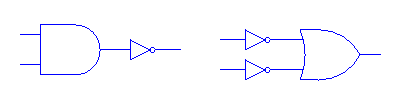
\includegraphics{figures/DeMorgan}}
}

\item Find the negation of each of the following and simplify as much as possible.
\medskip

  \begin{enumerate}
  \item $(A \lor B) \; \iff \; C$
\medskip

  \item $(A \lor B) \; \implies \; (A \land B)$

  \end{enumerate}

\wbvfill

\hint{Neither of these is particularly amenable to simplification. Nor, perhaps, is it readily
apparent what ``simplify'' means in this context! My interpretation is that we should look
for a logically equivalent expression using the fewest number of operators and if possible
{\em not} using the more complicated operators ($\implies$ and $\iff$).  However, if we try 
to rewrite the first statement's negation using only $\land$, $\lor$ and $\lnot$ we get things
that look a lot more complicated than $(A \lor B) \; \iff \; {\lnot}C$ -- the quick way to negate a 
bicondiitonal is simply to negate one of its parts.

The second statement's negation turns out to be the same thing as exclusive or, so a particularly
simple response would be to write $A \oplus B$ although that feels a bit like cheating, so
maybe we should answer with $(A \lor B) \land {\lnot}(A \land B)$ -- but that answer is what we
would get by simply applying the rule for negating a conditional and doing no further simplification.
}

\workbookpagebreak

\item Because a conditional sentence is equivalent to a certain disjunction, and 
because DeMorgan's law tells us that the negation of a disjunction is a conjunction,
it follows that the negation of a conditional is a conjunction.  Find denials (the negation
of a sentence is often called its ``denial'') for each of the following conditionals.

\begin{enumerate}
\item ``If you smoke, you'll get lung cancer.''
\item ``If a substance glitters, it is not necessarily gold.''
\item ``If there is smoke, there must also be fire.''
\item ``If a number is squared, the result is positive.''
\item ``If a matrix is square, it is invertible.''
\end{enumerate}

\wbvfill

\hint{
\begin{enumerate}
\item ``You smoke and you haven't got lung cancer.''
\item ``A substance glitters and it is necessarily gold.''
\item ``There is smoke,and there isn't fire.''
\item ``A number is squared, and the result is not positive.''
\item ``A matrix is square and it is not invertible.''
\end{enumerate}
}

\hintspagebreak
\workbookpagebreak

\item The so-called ``ethic of reciprocity'' is an idea that has come 
up in many of the world's religions and philosophies.  
Below are statements of the ethic
from several sources.  Discuss their logical meanings and determine which (if 
any) are logically equivalent.

\begin{enumerate}
\item ``One should not behave towards others in a way which is disagreeable to oneself.'' Mencius Vii.A.4 (Hinduism)
\item ``None of you [truly] believes until he wishes for his brother what he wishes for himself.'' Number 13 of Imam ``Al-Nawawi's Forty Hadiths.'' (Islam)
\item ``And as ye would that men should do to you, do ye also to them likewise.'' Luke 6:31, King James Version. (Christianity)
\item ``What is hateful to you, do not to your fellow man. This is the law: all the rest is commentary.'' Talmud, Shabbat 31a. (Judaism)
\item ``An it harm no one, do what thou wilt'' (Wicca)
\item ``What you would avoid suffering yourself, seek not to impose on others.'' (the Greek philosopher Epictetus -- first century A.D.)
\item ``Do not do unto others as you expect they should do unto you. Their tastes may not be the same.'' (the Irish playwright George Bernard Shaw -- 20th century A.D.)
\end{enumerate}

\wbvfill

\hint{
The ones from Wicca and George Bernard Shaw are just there for laughs.

For the remainder, you may want to contrast how restrictive they seem. For example the Christian version is (in my opinion) a lot stronger than the one from the Talmud -- ``treat others as you would want to be treated'' restricts your actions both in terms of what you would like done to you and in terms of what you wouldn't like done to you; ``Don't treat your fellows in a way that would be hateful to you.'' is leaving you a lot more freedom of action, since it only prohibits you from doing those things you wouldn't want done to yourself to others. The Hindus, Epictetus and the Jews (and the Wiccans for that matter) seem to be expressing roughly the same sentiment -- and promoting an ethic that is rather more easy for humans to conform to!

From a logical perspective it might be nice to define open sentences:

\[ W(x,y) \; = \; \mbox{``x would want y done to him.''} \]

\[ N(x,y)  \; = \; \mbox{``x would not want y done to him.''} \]

\[ D(x,y)  \; = \; \mbox{``do y to x.''} \]

\[ DD(x,y)  \; = \; \mbox{``don't do y to x.''} \]

In which case, the aphorism from Luke would be

\[ (W(you, y) \implies  D(others, y)) \land (N(you, y) \implies DD(others, y)) \]

}

\workbookpagebreak
\textbookpagebreak

\item You encounter two natives of the land of knights and knaves. Fill
in an explanation for each line of the proofs of their identities. 

\begin{enumerate}
\item Natasha says, ``Boris is a knave.'' \\
Boris says, ``Natasha and I are knights.''\\

\hintspagebreak

\textbf{Claim:} Natasha is a knight, and Boris is a knave.\\

\begin{proof} If Natasha is a knave, then Boris is a knight.\\
If Boris is a knight, then Natasha is a knight.\\
Therefore, if Natasha is a knave, then Natasha is a knight.\\
Hence Natasha is a knight.\\
Therefore, Boris is a knave.
\end{proof}

\item Bonaparte says ``I am a knight and Wellington is a knave.''\\
Wellington says ``I would tell you that B is a knight.''

\textbf{Claim:} Bonaparte is a knight and Wellington is a knave.

\begin{proof}
    Either Wellington is a knave or Wellington is a knight.\\
    If Wellington is a knight it follows that Bonaparte is a knight.\\
    If Bonaparte is a knight then Wellington is a knave. \\
    So, if Wellington is a knight then Wellington is a knave (which is impossible!)\\
    Thus, Wellington is a knave.\\
    Since Wellington is a knave, his statement ``I would tell you that Bonaparte is a knight'' is false. \\
    So Wellington would in fact tell us that Bonaparte is a knave. \\
    Since Wellington is a knave we conclude that Bonaparte is a knight.\\
    Thus Bonaparte is a knight and Wellington is a knave (as claimed).\\
\end{proof}

\hintspagebreak
\wbvfill

\hint{
Here's the second one:

\begin{proof}
    Either Wellington is a knave or Wellington is a knight.\\
    \rule{0pt}{0pt} \hfill \parbox{3in}{\color[rgb]{1,0,0} It's either one thing or the other! }\\
    If Wellington is a knight it follows that Bonaparte is a knight.\\
    \rule{0pt}{0pt} \hfill \parbox{3in}{\color[rgb]{1,0,0} That's what he said he would tell us and if he's a knight we can trust him.}\\
    If Bonaparte is a knight then Wellington is a knave. \\
    \rule{0pt}{0pt} \hfill \parbox{3in}{\color[rgb]{1,0,0} True, because that is one of the things Bonaparte states.}\\
    So, if Wellington is a knight then Wellington is a knave (which is impossible!)\\
    \rule{0pt}{0pt} \hfill \parbox{3in}{\color[rgb]{1,0,0} This is just summing up what was deduced above.}\\
    Thus, Wellington is a knave.\\
    \rule{0pt}{0pt} \hfill \parbox{3in}{\color[rgb]{1,0,0}  Because the other possibility leads to something {\em im}possible.}\\
    Since Wellington is a knave, his statement ``I would tell you that Bonaparte is a knight'' is false. \\
    \rule{0pt}{0pt} \hfill \parbox{3in}{\color[rgb]{1,0,0} Knave's statements are always false!}\\
    So Wellington would in fact tell us that Bonaparte is a knave. \\
    \rule{0pt}{0pt} \hfill \parbox{3in}{\color[rgb]{1,0,0} He was lying when he said he would tell us B is a knight.} \\
    Since Wellington is a knave we conclude that Bonaparte is a knight.\\
    \rule{0pt}{0pt} \hfill \parbox{3in}{\color[rgb]{1,0,0} Wait, now I'm confused\ldots can you do this part?} \\
    Thus Bonaparte is a knight and Wellington is a knave (as claimed).\\
    \rule{0pt}{0pt} \hfill \parbox{3in}{\color[rgb]{1,0,0} Just summarizing.} \\
\end{proof}

}

\end{enumerate}

\end{enumerate}


\newpage
\section{Two-column proofs}
\label{sec:2_col}

\noindent{\large \bf Exercises --- \thesection\ }

Write two-column proofs that verify each of the following
logical equivalences.

\begin{enumerate}
\item $A \lor (A \land B) \; \cong \; A \land (A \lor B)$
\medskip

\item $(A \land {\lnot}B) \lor A \; \cong \; A$
\medskip

\item $A \lor B \; \cong \; A \lor ({\lnot}A \land B)$
\medskip

\item ${\lnot}(A \lor {\lnot}B) \lor ({\lnot}A \land {\lnot}B) \; \cong \; {\lnot}A$
\medskip

\item $A \; \cong \; A \land ((A \lor {\lnot}B) \lor (A \lor B))$
\medskip

\item $(A \land {\lnot}B) \land ({\lnot}A \lor B) \; \cong \; c$
\medskip

\item $A \; \cong \; A \land (A \lor (A \land (B \lor C)))$
\medskip

\item ${\lnot}(A \land B) \land {\lnot}(A \land C) \; \cong \; {\lnot}A \lor ({\lnot}B \land {\lnot}C)$
\medskip

\end{enumerate}

\hint{
Here's the last one:

\begin{proof}

$  {\lnot}(A \land B) \land {\lnot}(A \land C) $ \\  
 \rule{0pt}{0pt} \hfill \parbox{3in}{\color[rgb]{1,0,0}  	 DeMorgan's law (times 2)} \\
$\equiv  \quad   ({\lnot}A \lor {\lnot}B) \land ({\lnot}A \lor {\lnot}C)	$ \\   
 \rule{0pt}{0pt} \hfill \parbox{3in}{\color[rgb]{1,0,0}  	 Distributive law} \\ 
$\equiv  \quad  {\lnot}A \lor ({\lnot}B \land {\lnot}C) $ \\  
\end{proof}

}
\workbookpagebreak

\rule{0pt}{0pt}

\workbookpagebreak

\newpage

\section{Quantified statements}
\label{sec:quant}

\noindent{\large \bf Exercises --- \thesection\ }

\begin{enumerate}
\item There is a common variant of the existential quantifier,
$\exists !$, if you write $\exists ! \, x, \, P(x)$ you are asserting 
that there is a \index{unique existence}\emph{unique} element 
in the universe that makes $P(x)$ true.
Determine how to negate the sentence $\exists ! \, x, \, P(x)$.

\hint{
Unique existence is essentially saying that there is exactly 1 element of the universe of discourse that makes P(x) true. The negation of "there is exactly 1" is "there's either none, or at least 2".

Is that enough of a hint?
}

\item The order in which quantifiers appear is important.  Let $L(x,y)$
be the open sentence ``$x$ is in love with $y$.''  Discuss the meanings of the
following quantified statements and find their negations.

\begin{enumerate}
\item $\forall x \, \exists y \; L(x,y)$.
\item $\exists x \, \forall y \; L(x, y)$.
\item $\forall x \, \forall y \; L(x, y)$.
\item $\exists x \, \exists y \; L(x, y)$.
\end{enumerate}

\hint{

\begin{enumerate}
\item $\forall x \, \exists y \; L(x,y)$.

This is a fairly optimistic statement  ``For everyone out there, there's somebody that they are in love with.''

\item $\exists x \, \forall y \; L(x, y)$.

This one, on the other hand, says something fairly strange: ``There's someone who has fallen in love with every other human being.'' I don't know, maybe the Dalai Lama? Mother Theresa?...
Anyway, do the last two for yourself.

\item $\forall x \, \forall y \; L(x, y)$.
\item $\exists x \, \exists y \; L(x, y)$.

\vspace{.5in}

Here's a couple of bonus questions. Two of the statements above have different meanings if you just interchange the order that the quantifiers appear in. What do the following mean (in contrast to the ones above)?

\item $\exists y \, \forall x \; L(x, y)$.
\item $\forall y \, \exists x \; L(x,y)$.
\end{enumerate}

}

\item Determine a useful denial of: 

$\displaystyle \forall \epsilon>0 \, \exists 
\delta>0 \, \forall x \, (|x-c| < \delta) \implies (|f(x)-l| < \epsilon) $.

The denial above gives a criterion for saying $\lim_{x\rightarrow c}f(x) \neq l.$

\hint{
This is asking you to put a couple of things together. The first thing is that in negating a quantified statement, we get a new statement with all the quantified variables occurring in the same order but with $\forall$'s and $\exists$'s interchanged. The second issue is that the logical statement that appears after all the quantifiers needs to be negated. Since, in this statement we have a conditional, you must remember to negate that properly (its negation is a conjunction).

$\displaystyle \exists \epsilon>0 \, \forall 
\delta>0 \, \exists x \, (|x-c| < \delta)  \land  (|f(x)-l| \geq \epsilon) $.

}

\item A \index{Sophie Germain prime} \emph{Sophie Germain prime} is a prime number $p$
such that the corresponding odd number $2p+1$ is also a prime.  For example 11 is a 
Sophie Germain prime since $23 = 2\cdot 11 + 1$ is also prime.  Almost all Sophie Germain
primes are congruent to $5 \pmod{6}$, nevertheless, there are exceptions -- so the
statement ``There are Sophie Germain primes that are not 5 mod 6.'' is true.  Verify this.

\hint{The exceptions are very small prime numbers. You should be able to find them easily.}

\item  Alvin, Betty, and Charlie enter a cafeteria which offers three different
entrees, turkey sandwich, veggie burger, and pizza; four different
beverages, soda, water, coffee, and milk; and two types of desserts,
pie and pudding. Alvin takes a turkey sandwich, a soda, and a pie.
Betty takes a veggie burger, a soda, and a pie. Charlie takes a pizza
and a soda. Based on this information, determine whether the following
statements are true or false.

\begin{enumerate}
\item \label{negated}$\forall$ people $p$, $\exists$ dessert $d$ such that $ p$
took $d$. \hint{false}
\item \label{compare}$\exists$ person $p$ such that $\forall$ desserts
$d$, $p$ did not take $d$. \hint{true}
\item $\forall$ entrees $e$, $\exists$ person $p$ such that $ p$ took
$e$. \hint{true}
\item \label{entree}$\exists$ entree $e$ such that  $\forall$ people
$p,\ p$ took $e$. \hint{false}
\item $\forall$ people $p$, $p$ took a dessert $\iff p$ did not take
a pizza. \hint{true}
\item Change one word of statement \ref{entree} so that it becomes true. \hint{entree $\longrightarrow$ beverage}
\item Write down the negation of \ref{negated} and compare it to statement
\ref{compare}. Hopefully you will see that they are the same! Does
this make you want to modify one or both of your answers to \ref{negated}
and \ref{compare}? \hint{$\exists$ person $p$ such that $\forall$ desserts
$d$, $p$ did not take $d$. Yes I do.  No, I got them right in the first place!}
\end{enumerate}

\end{enumerate}


\newpage

\section{Deductive reasoning and Argument forms}
\label{sec:deduct}

\noindent{\large \bf Exercises --- \thesection\ }

\begin{enumerate}

\item In the movie ``Monty Python and the Holy Grail'' we encounter
a medieval villager who (with a bit of prompting) makes the 
following argument.

\begin{quote}
If she weighs the same as a duck, then she's made of wood. \newline
If she's made of wood then she's a witch. \newline
Therefore, if she weighs the same as a duck, she's a witch.
\end{quote} 

Which rule of inference is he using?

\hint{
This is what many people refer to as the transitive rule of implication.  As an argument form it's known as ``hypothetical syllogism.''
}

\item In constructive dilemma, the antecedent of the conditional 
sentences are usually chosen to represent opposite alternatives. 
This allows us to introduce their disjunction as a tautology. 
Consider the following proof that there is never any reason to worry
(found on the walls of an Irish pub).

\begin{quote}
Either you are sick or you are well. \newline
If you are well there's nothing to worry about. \newline
If you are sick there are just two possibilities: \newline
Either you will get better or you will die. \newline
If you are going to get better there's nothing to worry about. \newline
If you are going to die there are just two possibilities:\newline
Either you will go to Heaven or to Hell. \newline
If you go to Heaven there is nothing to worry about.
If you go to Hell, you'll be so busy shaking hands with all your friends there won't be time to worry \ldots
\end{quote}

Identify the three tautologies that are introduced in this ``proof.''

\hint{Look at the lines that start with the word "Either."}

\textbookpagebreak

\item For each of the following arguments, write it in symbolic form and determine 
which rules of inference are used.

\begin{enumerate}
\item \rule{0pt}{24pt} You are either with us, or you're against us.  And you don't appear to be with us.
So, that means you're against us!

\hint{
\begin{center}
\begin{tabular}{cl}
 & $W \lor A$ \\
 & ${\lnot}W$ \\ \hline
$\therefore$ & $A$ \\
\end{tabular}
\end{center}

This is ``disjunctive syllogism.''
}


\item \rule{0pt}{24pt} All those who had cars escaped the flooding.  Sandra had a car -- therefore, Sandra
escaped the flooding.

\hint{
Let $C(x)$ be the open sentence ``x has a car'' and let $E(x)$ be the open sentence ``x escaped the flooding.''
This argument is actually the particular form of universal modus ponens: (See the final question in the next set of exercises.)

\begin{center}
\begin{tabular}{cl}
 & $\forall x, C(x) \implies E(x)$ \\
 & $C(\mbox{Sandra}) $ \\ \hline
$\therefore$ & $E(\mbox{Sandra})$ \\
\end{tabular}
\end{center}

At this stage in the game it would be perfectly fine to just identify this as modus ponens and not worry about the quantifiers that appear.
}

\item \rule{0pt}{24pt}  When Johnny goes to the casino, he always gambles 'til he goes broke.  Today, Johnny
has money, so Johnny hasn't been to the casino recently.
\item \rule{0pt}{24pt} (A non-constructive proof that there are 
irrational numbers $a$ and $b$ such that $a^b$ is rational.)  
Either $\sqrt{2}^{\sqrt{2}}$ is rational or it is irrational.
If $\sqrt{2}^{\sqrt{2}}$ is rational, we let $a=b=\sqrt{2}$.
Otherwise, we let $a=\sqrt{2}^{\sqrt{2}}$ and $b=\sqrt{2}$.
(Since $\sqrt{2}^{\sqrt{2}^{\sqrt{2}}} = 2$, which is rational.) It follows that in either case, there
are irrational numbers $a$ and $b$ such that $a^b$ is rational.


\end{enumerate}

\hint{I'm leaving the last two for you to do. One small hint: both are valid forms.}


\end{enumerate}


\newpage

\section{Validity of arguments and common errors}
\label{sec:valid}

\noindent{\large \bf Exercises --- \thesection\ }

\begin{enumerate}
\item Determine the logical form of the following arguments.  Use symbols
to express that form and determine whether the form is valid or invalid.
If the form is invalid, determine the type of error made.  Comment on the 
soundness of the argument as well, in particular, determine whether any of
the premises are questionable.
\begin{enumerate}
\item All who are guilty are in prison. \newline
  George is not in prison.  \newline
  Therefore, George is not guilty.
 
  \hint{ 
  This looks like modus tollens. Let $G$ refer to ``guilt'' and $P$ refer to ``in prison''
  
\begin{center}
\begin{tabular}{cl}
 & $\forall x, G(x) \implies P(x)$ \\
 & ${\lnot}P(\mbox{George}) $ \\ \hline
$\therefore$ & ${\lnot}G(\mbox{George})$ \\
\end{tabular}
\end{center}

You should note that while the form is valid, there is something terribly wrong with this argument. Is it really true that everyone who is guilty of a crime is in prison?
}

\item If one eats oranges one will have high levels of vitamin C. \newline
  You do have high levels of vitamin C. \newline
  Therefore, you must eat oranges.
\item All fish live in water. \newline
  The mackerel is a fish. \newline
  Therefore, the mackerel lives in water. 
\item If you're lazy, don't take math courses.\newline
  Everyone is lazy. \newline
  Therefore, no one should take math courses.
\item All fish live in water. \newline
  The octopus lives in water. \newline
  Therefore, the octopus is a fish.
\item If a person goes into politics, they are a scoundrel.\newline
  Harold has gone into politics. \newline
  Therefore, Harold is a scoundrel. 
\end{enumerate}

\item Below is a rule of inference that we call extended elimination.

\begin{tabular}{cl}
 & $(A \lor B) \lor C$ \\
 & ${\lnot}A$ \\
 & ${\lnot}B$ \\ \hline
$\therefore$ & $C$ \\
\end{tabular}

Use a truth table to verify that this rule is valid.

\hint{

\vfill

In the following truth table the predicate variables occupy the first 3 columns, the argument's 
premises are in the next three columns and the conclusion is in the right-most column.  The
truth values have already been filled-in.  You only need to identify the critical rows and 
verify that the conclusion is true in those rows.

\vfill

 \newpage
 
\begin{tabular}{|c|c|c||c|c|c||c|} \hline
\rule[-8pt]{0pt}{30pt}$A$ & $B$ & $C$ & $(A \lor B) \lor C$ & \rule{20pt}{0pt} ${\lnot}A$ \rule{20pt}{0pt} & \rule{20pt}{0pt} ${\lnot}B$ \rule{20pt}{0pt} & \rule{20pt}{0pt} $C$ \rule{20pt}{0pt} \\ \hline
\rule[-8pt]{0pt}{30pt}$T$ & $T$ & $T$ & $T$ & $\phi$ & $\phi$ & $T$  \\ \hline
\rule[-8pt]{0pt}{30pt}$T$ & $T$ & $\phi$  & $T$ & $\phi$ & $\phi$ & $\phi$   \\ \hline
\rule[-8pt]{0pt}{30pt}$T$ & $\phi$  & $T$ & $T$ & $\phi$ & $T$  & $T$  \\ \hline
\rule[-8pt]{0pt}{30pt}$T$ & $\phi$  & $\phi$  & $T$ & $\phi$ & $T$ & $\phi$   \\  \hline
\rule[-8pt]{0pt}{30pt}$\phi$  & $T$ & $T$ & $T$ & $T$ & $\phi$ &  $T$ \\ \hline
\rule[-8pt]{0pt}{30pt}$\phi$  & $T$ & $\phi$  & $T$ & $T$ & $\phi$ & $\phi$  \\ \hline
\rule[-8pt]{0pt}{30pt}$\phi$  & $\phi$  & $T$ & $T$ & $T$ & $T$ & $T$  \\ \hline
\rule[-8pt]{0pt}{30pt}$\phi$  & $\phi$  & $\phi$  & $\phi$ & $T$ & $T$ & $\phi$  \\  \hline
\end{tabular}

\vfill
}

\item If we allow quantifiers and open sentences in an argument form we
get a couple of new argument forms.  Arguments involving existentially quantified 
premises are rare -- the new forms we are speaking of are called ``universal modus 
ponens'' and ``universal modus tollens.''   The minor premises may also be quantified
or they may involve particular elements of the universe of discourse -- this leads
us to distinguish argument subtypes that are termed ``universal'' and ``particular.''

For example  \begin{tabular}{cl}
 & $\forall x, A(x) \implies B(x)$ \\
 & $A(p)$ \\ \hline
$\therefore$ & $B(p)$ \\
\end{tabular}  is the particular form of universal modus ponens (here, $p$
is not a variable -- it stands for some particular element of the universe of
discourse)
and \begin{tabular}{cl}
 & $\forall x, A(x) \implies B(x)$ \\
 & $\forall x, {\lnot}B(x)$ \\ \hline
$\therefore$ & $\forall x, {\lnot}A(x)$ \\
\end{tabular} is the universal form of (universal) modus tollens.

Reexamine the arguments from problem (1), determine their forms
(including quantifiers) and whether they are universal or particular.

\hint{
Hint: All of them except for one are the particular form -- number 4 is the exception.

Here's an analysis of number 5:

All fish live in water. \newline
The octopus lives in water.  \newline
Therefore, the octopus is a fish. \newline

Let $F(x)$ be the open sentence ``x is a fish'' and let $W(x)$ be the open sentence ``x lives in water.''

Our argument has the form

 \begin{center}
\begin{tabular}{cl}
 & $\forall x, F(x) \implies W(x)$ \\
 & $W(\mbox{the octopus}) $ \\ \hline
$\therefore$ & $F(\mbox{the octopus})$ \\
\end{tabular}
\end{center}

Clearly something is wrong -- a converse error has been made -- if everything that lived in water was necessarily a fish the argument would be OK (in fact it would then be the particular form of universal modus ponens).  But that is the converse of the major premise given.    
}

\item Identify the rule of inference being used.

\begin{enumerate}
\item The Buley Library is very tall.\\
Therefore, either the Buley Library is very tall or it has many
levels underground.

\hint{disjunctive addition}

\item The grass is green.\\
The sky is blue.\\
Therefore, the grass is green and the sky is blue.

\hint{conjunctive addition}

\item $g$ has order 3 or it has order 4.\\
If $g$ has order 3, then $g$ has an inverse.\\
If $g$ has order 4, then $g$ has an inverse.\\
Therefore, $g$ has an inverse.

\hint{constructive dilemma}

\item $x$ is greater than 5 and $x$ is less than 53.\\
Therefore, $x$ is less than 53.

\hint{conjunctive simplification}

\item If $a|b$, then $a$ is a perfect square.\\
If $a|b$, then $b$ is a perfect square.\\
Therefore, if $a|b$, then $a$ is a perfect square and $b$ is
a perfect square.

\hint{Note that the conclusion could be re-expressed as the conjunction of the two conditionals that
are found in the premises.  This is conjunctive addition with a bit of ``window dressing.''}
\end{enumerate}

\item Read the following proof that the sum of two odd numbers is even.
Discuss the rules of inference used.\\
\begin{proof}
Let $x$ and $y$ be odd numbers. Then $x=2k+1$
and $y=2j+1$ for some integers $j$ and $k$. By algebra,
\[
x+y = 2k+1 + 2j+1 = 2(k+j+1).
\]

Note that $k+j+1$ is an integer because $k$ and $j$ are integers.
Hence $x+y$ is even. 
\end{proof}

\hint{The definition for ``odd'' only involves the oddness of a single integer, but the first line of our
proof is a conjunction claiming that $x$ and $y$ are both odd.  It seems that two conjunctive simplifications, followed by applications of the definition, followed by a conjunctive addition have been used in order to
go from the first sentence to the second.}
 
\item Sometimes in constructing a proof we find it necessary to ``weaken'' an inequality.  For example,
we might have already deduced that $x < y$ but what we need in our argument is that $x \leq y$.  It is
okay to deduce $x \leq y$ from $x < y$ because the former is just shorthand for $x<y \lor x=y$.  What
rule of inference are we using in order to deduce that $x \leq y$ is true in this situation?

\hint{disjunctive addition}

\end{enumerate}


%% Emacs customization
%% 
%% Local Variables: ***
%% TeX-master: "GIAM-hw.tex" ***
%% comment-column:0 ***
%% comment-start: "%% "  ***
%% comment-end:"***" ***
%% End: ***

